\section{参数估计}
\label{sec:estimation}

\subsection{参考与度量}
\label{sec:reference}

全部常数都拟合自或反解自公开的 Mixbox~2.0 API \texttt{lerpFloat} 的输出测量，使用 sRGB 显示值浮点路径。参考从官方分发加载，仅供研究对照。度量为 CIEDE2000 \cite{sharma2005}，取 $k_{L}=k_{C}=k_{H}=1$，并对 Sharma 等的 34 组参考对做了验证（最大绝对偏差 $4.95\times10^{-5}$）。混合在显示值上进行，不做线性化；$\Delta E_{00}$ 在转换为 D65 下的 CIELAB 后计算。

\subsection{反解测量}
\label{sec:inversion}

设计由反解参考的测量驱动，而不是对颜料物理的假设。对每个锚点颜色对，在进度 $\alpha$ 处从参考输出读出幂律轨迹所需的逐通道指数：
\begin{equation}
p_{c}(\alpha)=\frac{\ln\bigl((r_{c}-v_{c})/(1-v_{c})\bigr)}{\ln\alpha},
\label{eq:inversion}
\end{equation}
其中 $v_{c}$ 为颜料通道值，$r_{c}$ 为参考输出。

由此得到三点结构观察（支撑数据见 \cref{app:inversion}）。第一，反解指数在 $\alpha$ 上近似恒定：各族在 $\alpha\in[0.1,0.9]$ 上的漂移小于 0.2，这支撑单指数模型；$\alpha\to1$ 附近的漂移由 $\varphi$ 映射处理。第二，指数随通道值呈两级下降——暗段保持吸收、亮段快速推进——这是 \cref{eq:staircase} 的经验依据。第三，残差结构依赖族与通道：近零通道依赖通道而非颜料；红族颜料亮化时保持其绿吸收；互补混合在区间中部留下近似 $4a(1-a)$ 形状的残差。这些观察引出 \cref{sec:repair} 的残差、耦合、方向与谐波项。

\Cref{fig:staircase} 绘出 $\alpha=0.5$ 处的反解指数、软阶跃近似，以及 PBM 输出的端到端反解。

\begin{figure}[t]
\centering
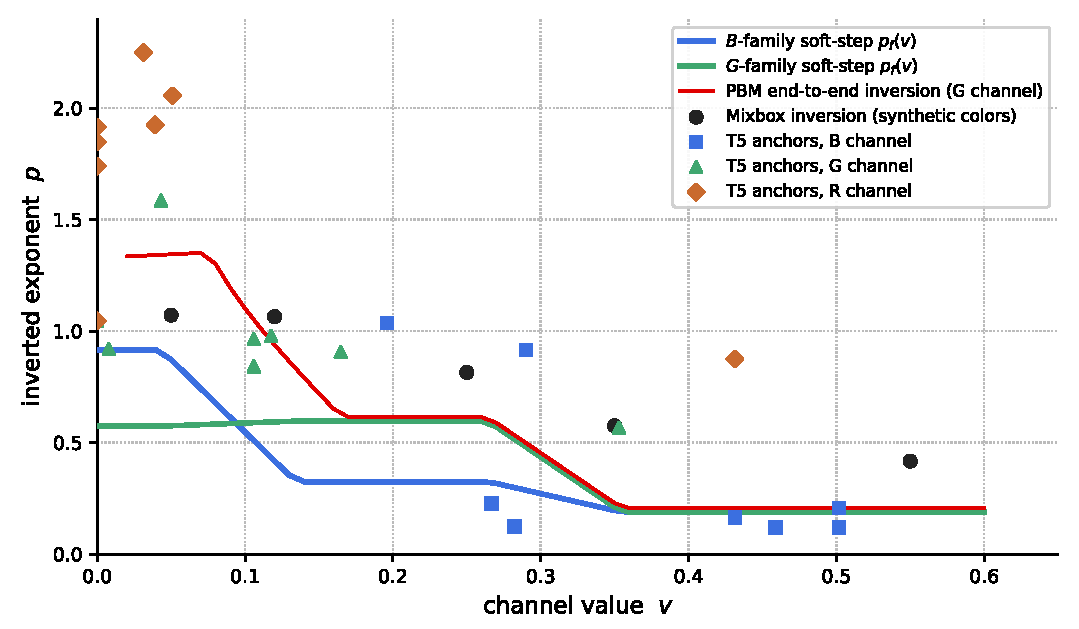
\includegraphics[width=0.78\linewidth]{fig3-staircase.pdf}
\caption{$\alpha=0.5$ 处的反解指数 $p$ 随通道值 $v$ 的变化。点：合成色与 T5 锚点的 Mixbox 反解。线：$B$、$G$ 族的软阶跃近似，以及 PBM 输出的端到端反解（G 通道）。}
\label{fig:staircase}
\end{figure}

\subsection{拟合流程}
\label{sec:fitting}

估计分两阶段，且可由仓库工具完整复现。

\paragraph{语料.}
拟合语料包含调色板套件（T1）、压力对套件（T2）、T3 抽样（seed 20260808）的前 800 个随机对、深色加白套件（T5）、双侧尾端套件（T5E）、6000 个伪随机 sRGB 对（seed 999），以及 12 个锚点互补色对（各取 19 个配比）；锚点对权重为 10，使谐波修正在其起作用处被拟合。

\paragraph{谐波系数.}
由于 $\hat{\gamma}$ 在 \cref{eq:harmonic} 中线性出现，51 个系数可闭式求得。对语料中每个条目，两个角色分支贡献
\begin{equation}
\mathbf{y}=
\mathbf{r}-\mathbf{C}-\sum_{b}\lambda_{b}\,g_{b}\,(T_{b}-\mathbf{C}),
\qquad
\mathbf{A}=\sum_{b}\lambda_{b}\,g_{b}\,V_{b},
\label{eq:design}
\end{equation}
其中 $\mathbf{r}$ 为参考输出，求和遍历当前的一个或两个分支；系数逐通道求解线性最小二乘 $\mathbf{A}\mathbf{w}\approx\mathbf{y}$，岭项取 $10^{-6}$。总增益 $\sum_{b}\lambda_{b}g_{b}$ 低于 0.02 的条目被排除，最终保留 4664 个设计行。

\paragraph{标量.}
其余十四个标量——两个阶梯位置、三个 $B$ 族水平与共享上台阶、耦合幅度与斜率、门控阈值/斜率/色度范围阈值、两个包络常数、端点压缩指数与残差幅度——在样本内损失上由坐标下降精修：
\begin{equation}
L=\overline{\Delta E_{00}}+0.02\,\max\Delta E_{00}+\frac{1}{12}\cdot\overline{\Delta E_{00}}\big|_{\text{锚点}},
\label{eq:loss}
\end{equation}
前两项在 T1、T2、T3 的 800 个拟合对与 T5 上求值。随后做一次交替：在更新后的核心上重拟合谐波系数，各套件变化小于 0.014 $\Delta E_{00}$，即两阶段已到达不动点。拟合得到的常数再在未参与拟合的留出抽样上复核（\cref{sec:results}）。

\paragraph{依测量证据采用的结构简化.}
阶梯斜率并入共享门控斜率；$G$ 与 $B$ 的上台阶共享同一值；$\varphi$ 宽度与 $E_{W}=0.08$ 共享；角色信号取最大通道；残差包络采用 \cref{eq:residual} 的 $C^{1}$ 二次式而非分段线性插值。

\subsection{门控敏感性}
\label{sec:sensitivity}

为检验门控阈值是否被调到狭窄的最优点，在固定其余参数的前提下，把每个门控阈值与共享斜率 $k$ 扰动 $\pm10\%$ 与 $\pm20\%$（\cref{tab:sensitivity}）。T5 的平均 $\Delta E_{00}$ 变化至多 0.11，T3 至多 0.05。T5 均值在 $w_{0}$ 与 $\mathrm{maxd}_{0}$ 扰动下基本不变，在 $k$ 缩放时最多移动 0.11；T3 最大值在 $w_{0}\times0.8$ 时从 19.4 升到 25.2，因为少数互补色对对门控边界敏感。因此这些阈值位于损失的平台上，而非刀刃上。

\begin{table}[t]
\centering
\small
\caption{门控参数敏感性：在固定其余参数时，对每个拟合门控参数施加 $\pm10\%$、$\pm20\%$ 扰动引起的平均 $\Delta E_{00}$ 变化（$\Delta$T5 / $\Delta$T3）。}
\label{tab:sensitivity}
\begin{tabular}{lcccc}
\toprule
参数 & $\times0.8$ & $\times0.9$ & $\times1.1$ & $\times1.2$ \\
\midrule
$w_{0}$（0.37375181） & $+0.000/-0.045$ & $+0.000/-0.023$ & $+0.000/+0.026$ & $+0.000/+0.081$ \\
$\mathrm{maxd}_{0}$（0.06479933） & $-0.011/-0.003$ & $-0.007/-0.002$ & $+0.010/+0.002$ & $+0.025/+0.005$ \\
共享斜率 $k$（11.0163945） & $+0.105/-0.001$ & $+0.029/-0.001$ & $+0.013/+0.002$ & $+0.038/+0.005$ \\
\bottomrule
\end{tabular}
\end{table}
